\section{Funzionamento di un display}
Questa sezione introduce il funzionamento di alcuni tipi di display moderni. Non è in alcun modo esaustiva, ma è utile conoscere le basi del funzionamento prima di continuare nei capitoli successivi.

Nel corso dei decenni, sono stati sviluppati innumerevoli tipi di display, ma le tecnologie più comunemente usate oggi sono LCD TFT e OLED: i primi sono più comuni sui PC, mentre i secondi si trovano prevalentemente sugli smartphone e i televisori.\\
Una differenza fondamentale tra un display OLED e un LCD TFT, è che i primi non hanno bisogno di retroilluminazione, poiché i pixel stessi emettono luce, mentre i secondi hanno bisogno di un qualche tipo di retroilluminazione poiché si basano su filtri che bloccano o lasciano passare la luce della retroilluminazione.\\
La retroilluminazione di un display LCD può essere realizzata in diversi modi: tradizionalmente si utilizzavano dei tubi a fluorescenza (CCFL) posizionati sui lati del display che illuminano un diffusore bianco generando una retroilluminazione più o meno uniforme; i tubi CCFL sono stati poi sostituiti da dei LED bianchi, posizionati sempre sui lati ad illuminare un diffusore; più recentemente i display di fascia alta hanno iniziato ad adottare un array di LED bianchi posizionati dietro al diffusore anziché sui lati, spesso individualmente controllabili per fornire un migliore contrasto (Full Array Local Dimming).\\
Con l'introduzione dei LED nella retroilluminazione, ci si scontra con il problema del dimming dei LED stessi: per simulare livelli bassi di luminosità, molti display, soprattutto quelli più economici, usano la tecnica della PWM (Pulse Width Modulation) per accendere e spegnere molto velocemente i LED creando l'illusione all'occhio umano di valori intermedi di luminosità. La frequenza più comune per la PWM è 240Hz, ma non è l'unica. Display di fascia più alta invece sono in grado di controllare il livello di luminosità dei LED in tensione o in corrente grazie a della circuiteria più sofisticata ma più costosa.

Davanti alla retroilluminazione, nei display LCD TFT, è presente una struttura che ha il compito di far passare o bloccare la luce alterando lo stato di uno strato di cristalli liquidi. Esistono principalmente tre tecnologie per fare questo, ognuna con i suoi vantaggi e svantaggi:
\begin{itemize}
	\item TN (Twisted Nematic): due filtri polarizzati di vetro sono posizionati rispettivamente dietro e davanti ad uno strato di cristalli liquidi, con una rotazione di 90°. Applicando una tensione allo strato di cristalli liquidi, si riesce ad alterarne la struttura in modo da variare la polarizzazione della luce che vi passa attraverso. A seconda della tensione applicata, passerà più o meno luce. Questo tipo di tecnologia è ancora oggi ampiamente utilizzata, soprattutto dai giocatori, per i bassi tempi di risposta, ma fornisce le peggiori prestazioni in termini di angolo di visione e qualità dell'immagine
	\item IPS (In-Plane Switching): a differenza dei display TN, i due filtri polarizzati sono paralleli e non ruotati di 90°. Per ottenere la rotazione di 90° del cristallo liquido, le parti interne del vetro dei due filtri sono trattate per allineare le molecole esterne del cristallo liquido alla giusta angolazione. Applicando una tensione con due elettrodi posizionati entrambi sullo stesso piano, si fa scorrere una corrente nel cristallo liquido essenzialmente parallela al piano, e si crea la rotazione che blocca o fa passare la luce. Questo è il tipo di tecnologia più utilizzata al momento, e fornisce la miglior qualità dell'immagine e angoli di visione, a scapito però di tempi di risposta relativamente alti, un maggior consumo di energia, costi più elevati, un nero poco profondo, e spesso una scarsa uniformità della retroilluminazione (detta backlight bleeding)
	\item VA (Vertical Alignment): simile a TN, ma i cristalli liquidi si allineano naturalmente in modo verticale ai filtri, bloccando il passaggio della luce. Applicando una tensione al cristallo liquido, questo si ruota verticalmente, permettendo a più o meno luce di passare in base alla tensione. Questa tecnologia è meno comune rispetto a IPS e TN, fornisce il miglior contrasto tra le tre, buoni tempi di risposta, e una qualità dell'immagine molto buona, seppur non ai livelli di un IPS; sfortunatamente è anche quella con l'angolo di visione più stretto, così stretto che una sorta di effetto tunnel sui bordi è pienamente visibile anche alla distanza e angolazione di utilizzo normale, motivo per cui è poco utilizzata
\end{itemize}

Dopo aver attraversato il cristallo liquido, la luce viene colorata da uno strato di filtri colorati detto maschera (mask) che contiene la matrice RGB che compone i pixel dello schermo.

Per controllare l'applicazione di tensione al cristallo liquido, delle linee di controllo verticale e orizzontale sono posizionate a matrice tra i pixel e permettono di controllare un TFT (Thin Film Transistor) presente in ogni subpixel. Questi piccolissimi transistor sono utilizzati per applicare la tensione al cristallo liquido.\\
I subpixel non sono indirizzabili individualmente (sarebbero necessarie troppe connessioni), il loro stato viene tipicamente aggiornato una linea per volta, ed è compito della matrice mantenere questo stato fino al refresh successivo usando un condensatore assieme al transistor per mantenere l'informazione mentre le altre linee vengono aggiornate. Questa tecnica prende il nome di active matrix (matrice attiva), e tutti i display TFT moderni usano questo tipo di matrice.

Alcuni display, soprattutto quelli più economici, non utilizzano tutta l'informazione presente nell'immagine in arrivo dalla scheda video per controllare i subpixel (ad esempio, su 8 bit per canale potrebbero usarne solo 6), così da avere una circuiteria più semplice e meno costosa, e compensano facendo uso di tecniche di dithering spaziale e/o temporale.

\begin{figure}[h]
	\centering
	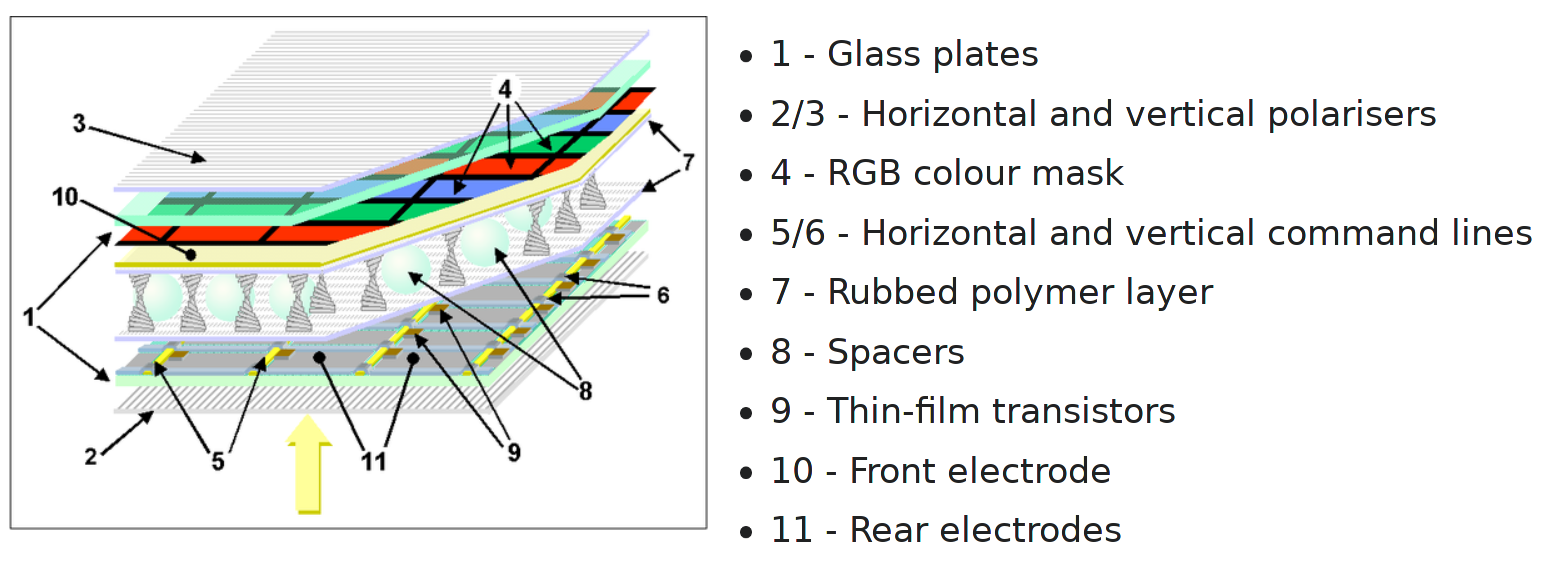
\includegraphics[width=\textwidth]{Chapter01/res/lcdtft.png}
	\caption{Struttura di un display LCD TFT (da Wikipedia, l'enciclopedia libera)}
	\label{fig:lcdtft}
\end{figure}

Per quanto riguarda i display OLED, le cose sono un po' più semplici: si tratta sostanzialmente di una matrice di piccolissimi LED organici controllati da una matrice attiva. Ogni LED è composto da due elettrodi, uno dei quali è trasparente, e nel mezzo è presente un polimero organico che emette luce quando viene applicata una tensione. Non richiedono retroilluminazione poiché i LED emettono luce propria anziché filtrarla, il che permette di creare display trasparenti con una buona visibilità, display flessibili, display estremamente sottili (ragione per cui sono comuni sugli smartphone). Il contrasto è eccezionale e i tempi di risposta sono buoni, tuttavia si usurano molto più velocemente rispetto ai display LCD TFT, anche se inutilizzati, l'usura non è uniforme nè nello spazio nè nei colori, soffrono di burn-in (ossia immagini statiche come loghi visualizzate a lungo restano impresse permanentemente sul display), e il polimero organico è estremamente vulnerabile ai liquidi e all'umidità.

\begin{figure}[h]
	\centering
	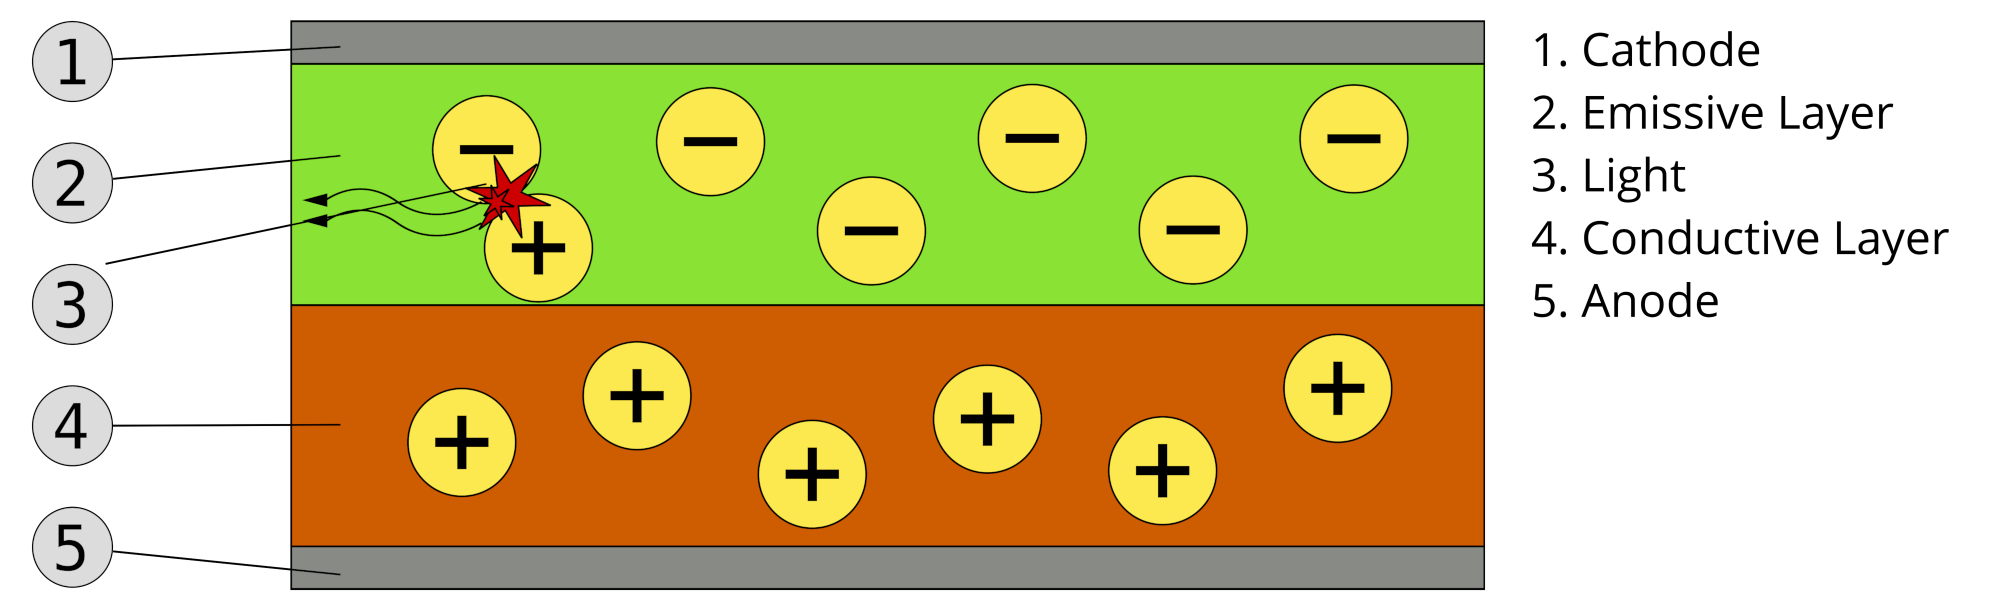
\includegraphics[width=\textwidth]{Chapter01/res/oled.png}
	\caption{Struttura di un subpixel OLED (da Wikipedia, l'enciclopedia libera)}
	\label{fig:oled}
\end{figure}

Il passo finale nella produzione del display è uno strato protettivo di vetro per progettere il tutto. Questo vetro può essere lucido per esaltare i colori, oppure avere una grana molto fine, per ridurre i riflessi.

Questo conclude la panoramica sulle tecnologie di display più comunemente utilizzate.

\subsection{Glossario}
In questa sezione vengono definiti in modo semplice e diretto alcuni termini relativi ai display che saranno utilizzati nel corso della tesi, oltre a quelli già definiti.

\textbf{Refresh rate}: la frequenza con cui vengono aggiornate le immagini sullo schermo. Tipicamente è 60 Hz.

\textbf{VRR}: Variable Refresh Rate, consente al display di variare il refresh rate entro un certo intervallo, consentendo alla GPU di inviare i fotogrammi quando sono pronti, riducendo il ritardo ed eliminando il tearing\todo{atrent: fai un glossario vero e proprio dei termini, in fondo al testo, ci sono pacchetti latex che te lo fanno!} senza bisogno di VSync. Lo standard si chiama VESA Adaptive Sync, i nomi commerciali sono Nvidia G-Sync e AMD Freesync.

\textbf{Tempo di risposta dei pixel}: il tempo in millisecondi che un pixel impiega per transizionare tra un colore e un altro. Esistono vari metodi per misurarlo.

\textbf{Overdrive}: una tecnica utilizzata per ridurre i tempi di risposta dei pixel "esagerando" le transizioni (per esempio, se si deve passare da 32 a 64, se per un breve istante si passa a 128 e poi si torna a 64 la transizione sarà più rapida). Overdrive eccessivo può causare artefatti visibili.

\textbf{Motion blur / Ghosting}: scia visibile dietro agli oggetti in movimento causata dai tempi di risposta dei pixel.

\textbf{Inverse ghosting}: artefatto creato dall'eccessivo overdrive, simile al ghosting, ma di colore opposto.

\textbf{PWM}: Pulse Width Modulation, lampeggio periodico della retroilluminazione per variare la luminosità.

\textbf{Strobing}: disattivazione intenzionale della retroilluminazione, tipicamente per nascondere le transizioni dei pixel.

\textbf{Black Frame Insertion}: tecnica adottata dai display a refresh rate molto alto (240Hz e più) per ridurre il motion blur percepito inserendo dei fotogrammi neri tra i fotogrammi di un segnale a frequenza inferiore.

\textbf{Contrasto dinamico}: tecnica adottata da alcuni display per variare il livello della retroilluminazione in base alla luminosità dell'immagine attualmente visualizzata. Permette di falsare un contrasto più elevato nei test.

\textbf{HDR / WGC}: High Dynamic Range e Wide Color Gamut. Indica la possibilità del display di visualizzare un range di luminosità e di colori più ampio rispetto al normale. In termini di marketing, tipicamente questo significa che il display è in grado di accettare un segnale RGB a 10 bit per canale nello spazio colore BT.2020. Esistono diversi standard che lo definiscono nel dettaglio, come HDR10 e Dolby Vision, e certificazioni come VESA DisplayHDR che indicano i livelli minimi di luminosità che un display deve avere per essere definito HDR.

\textbf{Local Dimming}: tecnica simile al contrasto dinamico, ma anziché variare la luminosità dell'intero schermo, può variare solo determinate zone controllando individualmente i LED della retrolluminazione. Tende a creare aloni attorno agli oggetti luminosi.

%altro da aggiungere?
